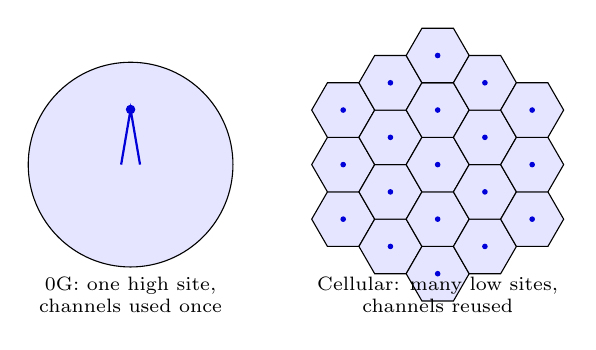
\begin{tikzpicture}[>=latex]
    \def\hexcell#1#2{\draw[fill=blue!10, shift={(#1,#2)}] (0:0.4) -- (60:0.4) -- (120:0.4) -- (180:0.4) -- (240:0.4) -- (300:0.4) -- cycle;}

    % 0G: one tower covers the whole area
    \draw[fill=blue!10] (0,0) circle (1.3);
    \draw[thick, blue!85!black] (-0.12,0) -- (0,0.7) -- (0.12,0);
    \filldraw[blue!85!black] (0,0.7) circle (1.5pt);
    \node[font=\scriptsize, align=center] at (0,-1.65) {0G: one high site,\\channels used once};

    % Cellular: many low sites
    \foreach \q in {-2,...,2} {
        \foreach \v in {-2,...,2} {
            \pgfmathtruncatemacro{\dist}{max(abs(\q),abs(\v),abs(\q+\v))}
            \ifnum\dist<3
                \pgfmathsetmacro{\cx}{3.9+0.6*\q}
                \pgfmathsetmacro{\cy}{0.6928*(\v+0.5*\q)}
                \hexcell{\cx}{\cy}
                \filldraw[blue!85!black] (\cx,\cy) circle (0.8pt);
            \fi
        }
    }
    \node[font=\scriptsize, align=center] at (3.9,-1.65) {Cellular: many low sites,\\channels reused};
\end{tikzpicture}
